\documentclass[10pt,a4paper]{article}

% ---------------------------------------------------------------------------
% Paquetes
% ---------------------------------------------------------------------------
\usepackage[utf8]{inputenc}
\usepackage[T1]{fontenc}
\usepackage[spanish,es-nodecimaldot]{babel}
\usepackage[a4paper, margin=2.5cm]{geometry}
\usepackage{graphicx}
\usepackage{float}
\usepackage{booktabs}
\usepackage{longtable}
\usepackage{array}
\usepackage{amsmath}
\usepackage[hidelinks]{hyperref}

\geometry{margin=2.5cm}
\graphicspath{
    {../../freq_meas/pics/}
    {../../prbs/pics/}
    {../../fir_parallel/pics/}
    {../../du/pics/}
    {../../regmap/pics/}
    {../pics/}
    {pics/}
}

% Reemplazar cada llamada a \pendiente por el contenido correspondiente.
\newcommand{\pendiente}[1]{\textit{[Completar: #1]}}

% ---------------------------------------------------------------------------
% Datos del informe
% ---------------------------------------------------------------------------
\begin{document}

\hypersetup{pageanchor=false}
\begin{titlepage}
\centering


\includegraphics[width=0.55\textwidth]{fulgor.png}

{\Huge\bfseries Trabajo Práctico N°2\par}
\vspace{0.5cm}
{\LARGE Generador PRBS, Filtro FIR, Unidad de Diagnóstico (DU), Medidor de Clock y Mapa de Registros\par}
\vspace{1.5cm}
{\Large Curso de Diseño Digital VLSI - Fundación Fulgor\par}
\vfill

{\Large Damián Lugano\par}
\vspace{0.5cm}
{\large \today\par}

\end{titlepage}

\hypersetup{pageanchor=true}
\pagenumbering{roman}
\tableofcontents
\clearpage
\pagenumbering{arabic}

% ---------------------------------------------------------------------------
\section{Introducción}
\label{sec:introduccion}
% ---------------------------------------------------------------------------

\subsection{Objetivos}
El objetivo de este trabajo es el diseño de un sistema capaz de generar un estímulo, 
procesarlo, y luego observarlo con una ventana de captura, todo controlado a través 
de un mapa  de registros, siendo este la única conexión entre el software y el 
hardware. Además,  este modulo integrará un modulo de medición de frecuencia, para 
chequear que la frecuencia del clock es la correcta.

\subsection{Arquitectura general}
El diseño contemplará 5 bloques principales, cada uno con una función definida.
Además, contará con 2 dominios de reloj: CPU y DSP. Cada modulo trabajará en un
dominio de clock, o incluso en los dos, por lo que este diseño integrará también,
multiples técnicas de CDC (Clock Domain Crossing).


\begin{figure} [H]
    \centering
    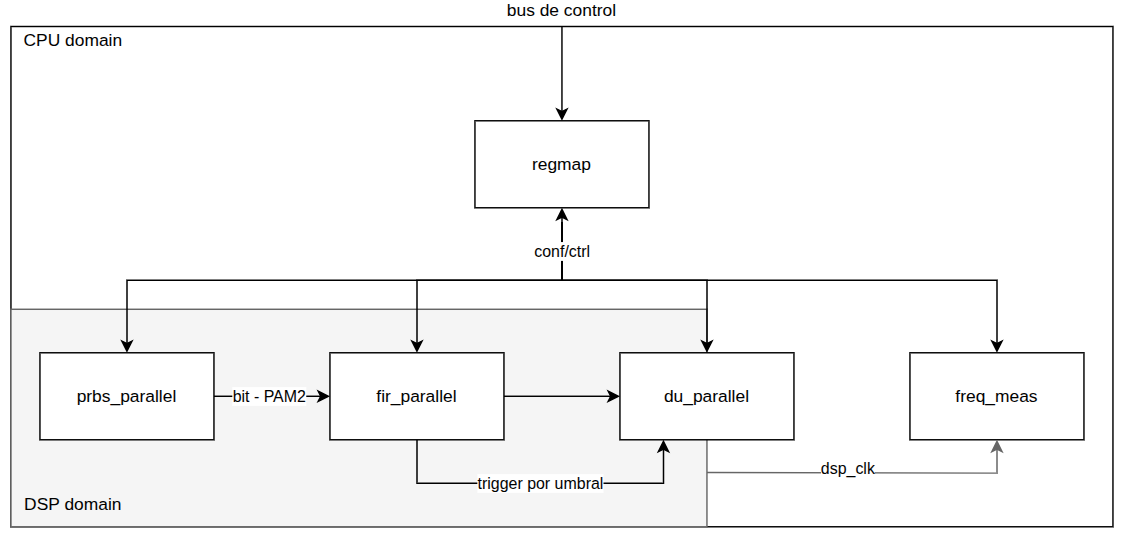
\includegraphics[width=\linewidth]{arquitectura_general.png}
    \caption{Esquema simple de la arquitectura general del sistema}
    \label{fig:arquitectura_general}
\end{figure}

\subsubsection*{Bloque A: Generador PRBS}
El generador PRBS es un generador de secuencias binarias pseudo-aleatorias basado en
un LFSR (Linear Feedback Shift Register). El mismo tendrá implementados 6 polinomios
de PRBS de 10 a 15, que podrán ser seleccionados mediante configuración desde el regmap.

En este caso, se hace una implementación paralela del generador PRBS, de 4 salidas.
La salida de este módulo será modulada a PAM-2 a traves de un submodulo y será el 
input del filtro FIR paralelo.

Su funcionamiento será principalmente en el clock DSP.

\subsubsection*{Bloque B: Filtro FIR}
Se utilizará el mismo filtro FIR del TP N°1, un filtro RRC(Root Raised Cosine) de 19 
taps, aunque en esta oportunidad se le hicieron modificaciones a su arquitectura para 
permitir una paralelización de 4.

Como entrada toma la secuencia pseudoaleatoria del PRBS modulada a PAM-2 y su salida 
irá a la DU para su visualización. Tanto sus coeficientes, como su señal de enable se 
configurarán mediante el regmap.

Su funcionamiento será principalmente en el clock DSP.

\subsubsection*{Bloque C: DU (Diagnostic Unit)}
Debe pensarse a la DU como un osciloscopio digital, dentro del mismo chip. Su 
funcionamiento se basa en capturar una señal a su entrada luego de su disparo, que 
será  en este caso por umbral.

Una vez disparado, en función de su modo de captura, tomará una cierta cantidad de 
muestras hasta completar su memoria. Luego de eso, su memoria podrá ser leida 
secuencialmente mediante  el regmap.

En este caso, al tratarse de una implementación paralela, se instanciarán 4 DUs, que 
se dispararáncon la misma señal de trigger en simultaneo y capturarán la señal de 
forma paralela en simultaneo.

Su funcionamiento será principalmente en el clock DSP, aunque la lectura de la memoria
será sincrónica al clock de CPU, para su lectura mediante el regmap.

\subsubsection*{Bloque D: Medidor de frecuencia de clock}
El medidor de frecuencia de clock es un modulo que, si bien no forma parte del 
datapath, es fundamental para la verificación de un clock de dominio desconocido, en 
base a uno conocido.

Brevemente, su funcionamiento se basa en dos contadores simultaneos, uno por cada 
dominio de clock, que contarán durante una ventana de tiempo de referencia generada a 
partir del clock conocido. Una vez terminada, se podrá calcular la relación entre 
cuentas del clock desconocido, y la ventana de tiempo configurada.

En este caso, el clock conocido o de referencia será el clock de CPU, mientras que el
clock a medir será el de DSP.

\subsubsection*{Bloque E: Mapa de registros}
El mapa de registros es la interfaz de entrada/salida entre el SW y el sistema en HW. 
Mediante el regmap, se podrá configurar, controlar y leer los resultados de todos
los modulos dentro del chip.

Su funcionamiento será principalmente en el clock de CPU, ya que es el nexo entre este
y el chip.

% ---------------------------------------------------------------------------
\section{Bloque A: Generador PRBS (\texttt{prbs\_parallel})}
\label{sec:prbs}
% ---------------------------------------------------------------------------

\subsection{Descripción y especificaciones}
El módulo implementado genera secuencias binarias pseudo-aleatorias mediante un
registro de desplazamiento con realimentación lineal (LFSR). El orden de la secuencia
es configurable entre PRBS10 y PRBS15 y el estado inicial se determina mediante una
semilla no nula, configurable.

Con el objetivo de paralelizar el sistema, el generador produce cuatro bits consecutivos 
de la secuencia PRBS en cada ciclo del clock DSP. Por lo tanto, el diseño posee un grado 
de paralelismo $P=4$. La selección del polinomio y la semilla se realizan desde el mapa 
de registros y son capturadas al inicio una nueva secuencia.

\subsubsection*{Polinomios implementados}

La Tabla~\ref{tab:prbs-polinomios} presenta los seis polinomios implementados y el
valor utilizado para seleccionarlos. Cada término del polinomio determina uno de los
taps que intervienen en la realimentación del LFSR. Las sumas se realizan en el campo
de Galois $\mathrm{GF}(2)$, por lo que se implementan mediante operaciones XOR.

\begin{table}[H]
    \centering
    \caption{Polinomios implementados por el generador PRBS.}
    \label{tab:prbs-polinomios}
    \begin{tabular}{ccc}
        \toprule
        \textbf{Selección} & \textbf{Patrón} & \textbf{Polinomio} \\
        \midrule
        \texttt{000} & PRBS10 & $x^{10}+x^7+1$ \\
        \texttt{001} & PRBS11 & $x^{11}+x^9+1$ \\
        \texttt{010} & PRBS12 & $x^{12}+x^6+x^4+x+1$ \\
        \texttt{011} & PRBS13 & $x^{13}+x^4+x^3+x+1$ \\
        \texttt{100} & PRBS14 & $x^{14}+x^5+x^3+x+1$ \\
        \texttt{101} & PRBS15 & $x^{15}+x^{14}+1$ \\
        \bottomrule
    \end{tabular}
\end{table}

\subsection{Paralelización del generador}

\subsubsection*{Representación matricial}
El comportamiento de un LFSR puede expresarse como un sistema lineal sobre
$\mathrm{GF}(2)$. Si $\mathbf{s}[k]$ representa su estado en el instante $k$ y $A$ es
la matriz de transición correspondiente al polinomio seleccionado, el avance de un
generador serial queda definido por

\begin{equation}
    \mathbf{s}[k+1] = A\,\mathbf{s}[k].
    \label{eq:prbs-transicion-serial}
\end{equation}

Para obtener $P$ bits por ciclo no es necesario instanciar cuatro veces el generador PRBS. 
En cambio, se eleva la matriz de transición a la potencia correspondiente al grado de paralelismo:

\begin{equation}
    \mathbf{s}[k+P] = A^P\,\mathbf{s}[k].
    \label{eq:prbs-transicion-paralela}
\end{equation}

En este diseño $P=4$, por lo que el próximo estado se calcula mediante $A^4$. Un
script desarrollado en Python construye la matriz $A$ a partir de los taps, se calcula
su cuarta potencia módulo 2 y permite obtener las ecuaciones XOR utilizadas en el
RTL.

\subsubsection*{Ejemplo para PRBS10}

Para mostrar el procedimiento se considera el polinomio de PRBS10

\begin{equation}
    p(x)=x^{10}+x^7+1.
\end{equation}

La matriz de transición es:

\begingroup
\scriptsize
\begin{equation}
A=
\begin{bmatrix}
0&0&0&0&0&0&1&0&0&1\\
1&0&0&0&0&0&0&0&0&0\\
0&1&0&0&0&0&0&0&0&0\\
0&0&1&0&0&0&0&0&0&0\\
0&0&0&1&0&0&0&0&0&0\\
0&0&0&0&1&0&0&0&0&0\\
0&0&0&0&0&1&0&0&0&0\\
0&0&0&0&0&0&1&0&0&0\\
0&0&0&0&0&0&0&1&0&0\\
0&0&0&0&0&0&0&0&1&0
\end{bmatrix}.
\label{eq:prbs10-matriz-serial}
\end{equation}
\endgroup

Al calcular la cuarta potencia de esta matriz en $\mathrm{GF}(2)$ se obtiene:

\begingroup
\scriptsize
\begin{equation}
A^4=
\begin{bmatrix}
0&0&0&1&0&0&1&0&0&0\\
0&0&0&0&1&0&0&1&0&0\\
0&0&0&0&0&1&0&0&1&0\\
0&0&0&0&0&0&1&0&0&1\\
1&0&0&0&0&0&0&0&0&0\\
0&1&0&0&0&0&0&0&0&0\\
0&0&1&0&0&0&0&0&0&0\\
0&0&0&1&0&0&0&0&0&0\\
0&0&0&0&1&0&0&0&0&0\\
0&0&0&0&0&1&0&0&0&0
\end{bmatrix}.
\label{eq:prbs10-matriz-paralela}
\end{equation}
\endgroup

Las filas de $A^4$ determinan las ecuaciones del próximo estado. Expresadas con la
numeración utilizada en el RTL resultan:

\begin{equation}
\begin{aligned}
q_9[k+4]&=q_5[k], & q_4[k+4]&=q_0[k],\\
q_8[k+4]&=q_4[k], & q_3[k+4]&=q_9[k]\oplus q_6[k],\\
q_7[k+4]&=q_3[k], & q_2[k+4]&=q_8[k]\oplus q_5[k],\\
q_6[k+4]&=q_2[k], & q_1[k+4]&=q_7[k]\oplus q_4[k],\\
q_5[k+4]&=q_1[k], & q_0[k+4]&=q_6[k]\oplus q_3[k].
\end{aligned}
\label{eq:prbs10-ecuaciones-paralelas}
\end{equation}

Los cuatro bits entregados durante el ciclo son $q_9[k]$, $q_8[k]$, $q_7[k]$ y
$q_6[k]$. Estos corresponden a cuatro valores consecutivos del generador PRBS.
Luego de presentarlos en la salida, el registro avanza directamente al estado
$\mathbf{s}[k+4]$. La Figura~\ref{fig:prbs10-paralelo} muestra el circuito resultante
para este polinomio.

\begin{figure}[H]
    \centering
    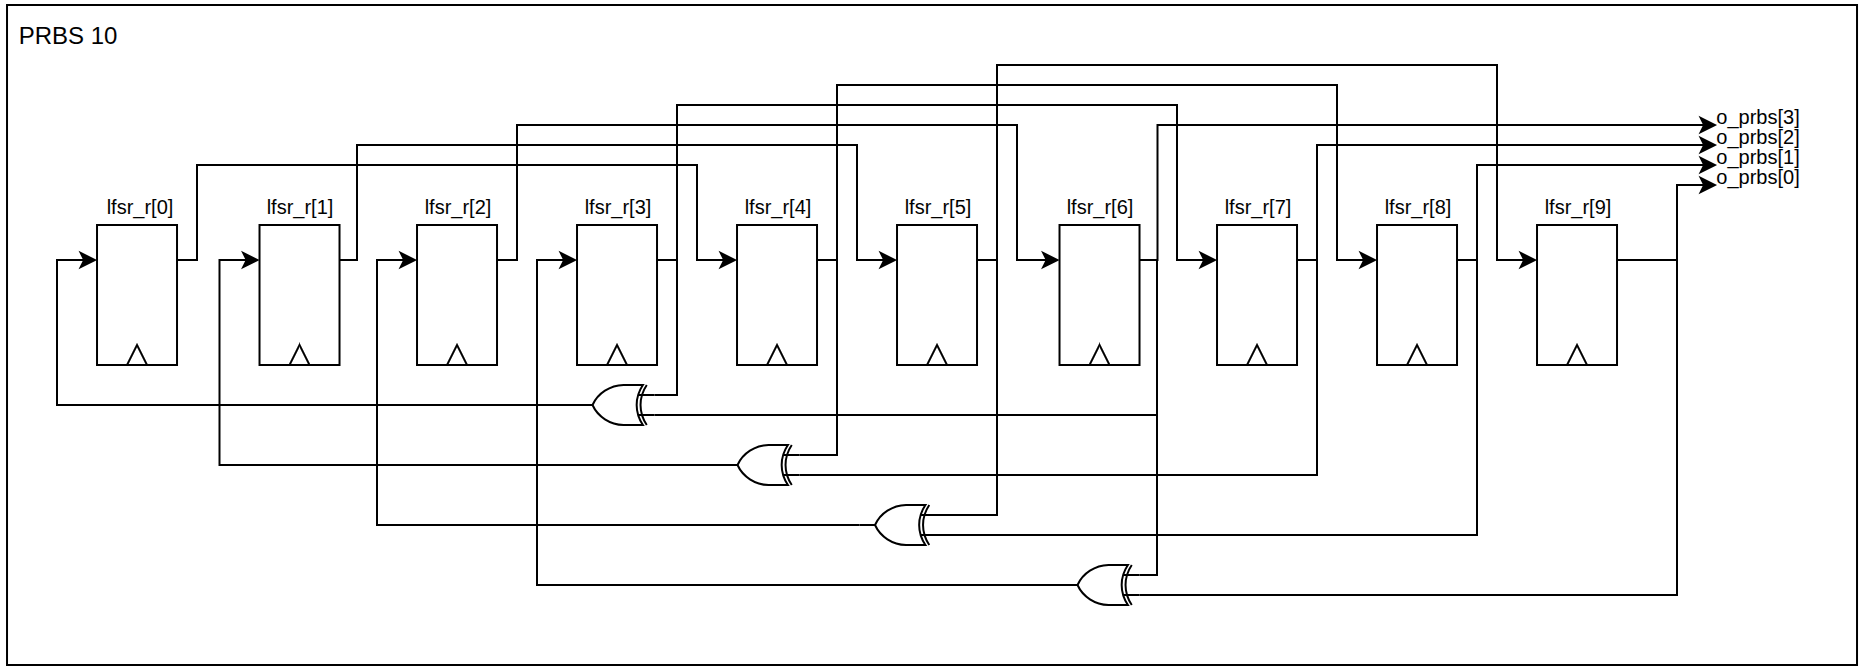
\includegraphics[width=\linewidth]{prbs10.png}
    \caption{Implementación paralela de grado cuatro para PRBS10.}
    \label{fig:prbs10-paralelo}
\end{figure}

\subsection{Implementación RTL}

El datapath utiliza un banco de registros de 15 bits, correspondiente al mayor orden 
soportado. Para cada polinomio seleccionado, el bloque combinacional calcula el 
próximo estado mediante las ecuaciones obtenidas de la matriz $A^4$. Los bits que no
pertenecen al orden seleccionado se mantienen fuera del estado activo. Por otro lado, 
otro bloque combinacional selecciona los cuatro bits más significativos del LFSR 
correspondiente y los presenta en las salidas paralelas.

La selección activa se almacena en \texttt{sel\_r}, el estado del LFSR en
\texttt{lfsr\_r} y la condición de ejecución en \texttt{running\_r}. La semilla y el
polinomio se capturan únicamente ante un pulso de inicio. Esto evita que una escritura
de configuración realizada mientras el generador está activo modifique la secuencia
en curso. La arquitectura RTL sintetizada se muestra en la
Figura~\ref{fig:prbs-arquitectura-rtl}.

\begin{figure}[H]
    \centering
    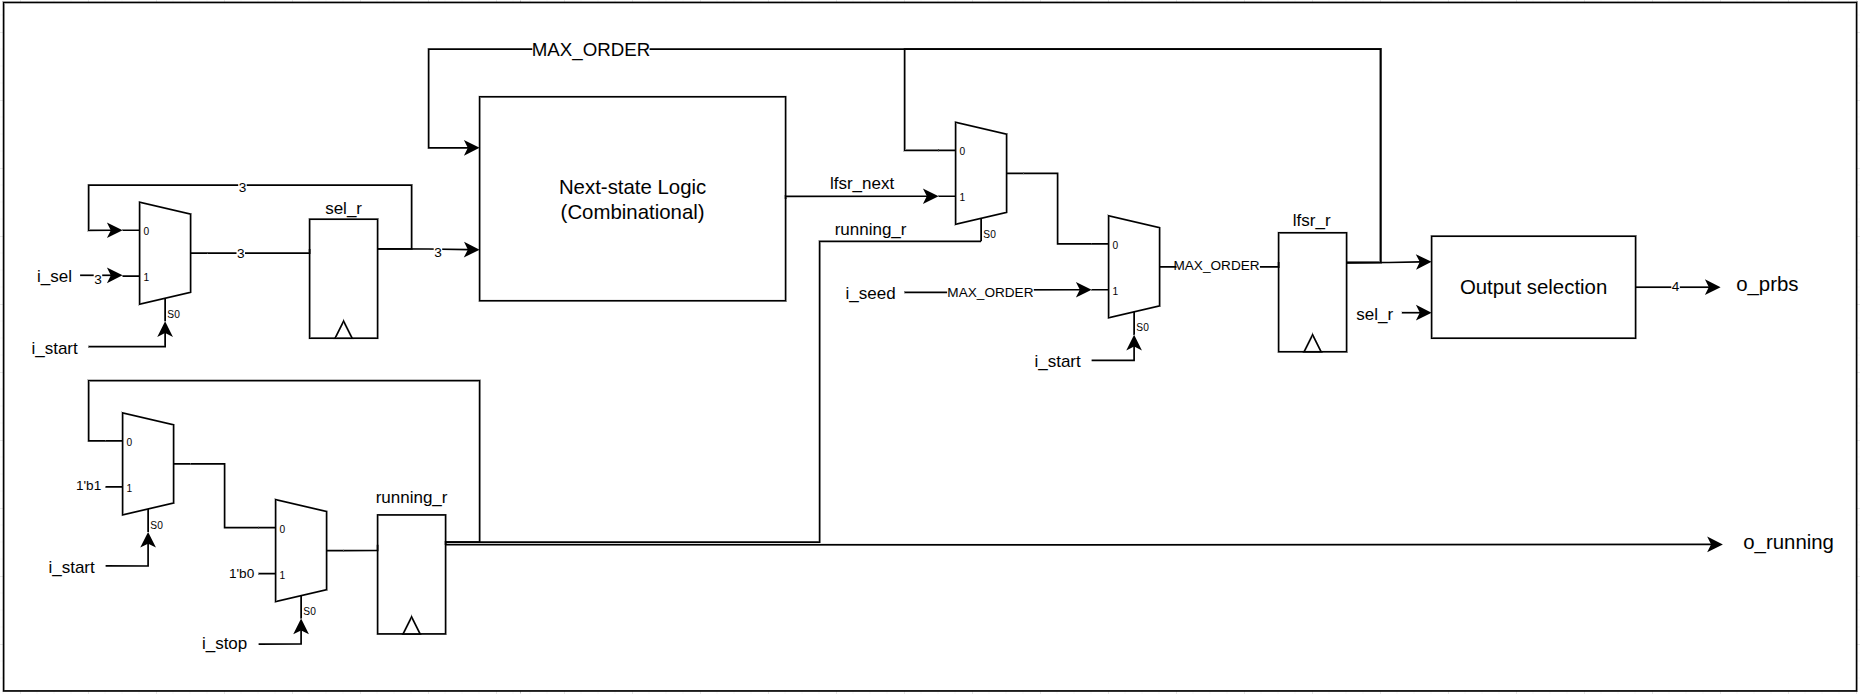
\includegraphics[width=\linewidth]{prbs_parallel_rtl.png}
    \caption{Arquitectura RTL del generador PRBS configurable.}
    \label{fig:prbs-arquitectura-rtl}
\end{figure}

\subsubsection*{Secuencia de configuración}

La configuración del generador debe realizarse antes de iniciar una secuencia. En
primer lugar se escribe una semilla no nula en \texttt{PRBS\_SEED}. Luego se escribe
en \texttt{PRBS\_CTRL[4:2]} la selección indicada en la
Tabla~\ref{tab:prbs-polinomios} y se genera un pulso de START mediante el bit 0 del
mismo registro. Al recibir este pulso en el dominio DSP, el módulo captura la semilla
y la selección, carga el estado inicial y activa \texttt{RUNNING}.

Mientras el generador se encuentra activo entrega cuatro bits y avanza cuatro
posiciones de la secuencia por cada ciclo. Para detenerlo se genera un pulso de STOP
mediante \texttt{PRBS\_CTRL[1]}. El estado queda congelado hasta recibir un nuevo
START, momento en el que se vuelven a cargar la configuración y la semilla. El estado
de ejecución puede consultarse en \texttt{PRBS\_STATUS[0]}.

\subsection{Verificación}

La verificación se realizó en dos partes. Inicialmente se realizó un testbench básico
para recorrer un período completo de cada uno de los polinomios implementados. Para
cada orden se usó una semilla con todos sus bits en uno. Las salidas del RTL se 
compararon bit a bit con secuencias generadas mediante un modelo de referencia 
desarrollado en Python.

Después, se implementó un testbench más robusto basado en clases y organizado con una
estructura tipo UVM. En este tesbench, se implementó: un generador que crea 
configuraciones aleatorias válidas de polinomio, semilla y duración; un driver que aplica 
la secuencia de reset, configuración, START y STOP; y un monitor que registra los cuatro 
bits producidos en cada ciclo. Finalmente, las muestras capturadas se comparan con el modelo 
de referencia de Python. 

De esta manera severificó tanto la correspondencia de las secuencias paralelas con el modelo serial
como el comportamiento de control del módulo frente a diferentes configuraciones.

% ---------------------------------------------------------------------------
\section{Bloque B: Filtro FIR (\texttt{fir\_parallel})}
\label{sec:fir}
% ---------------------------------------------------------------------------

\subsection{Descripción general}

Para el modulo de filtro FIR se utilizó el diseño del filtro RRC (Root Raised Cosine) de 19 
taps desarrollado en el TP1. Se conservó principalmente la arquitectura de la suma de 
productos del diseño original, que aprovechaba simetría y entrada PAM-2 utilizando 
arquitectura folded y muxes como multiplicadores.

Sin embargo, en este caso por el paralelismo implementado en el datapath, la entrada está 
compuesta por cuatro símbolos PAM-2 consecutivos y la salida contiene las cuatro muestras 
filtradas correspondientes.

La Figura~\ref{fig:fir-generico} presenta un FIR genérico de ocho taps. Este ejemplo
se utiliza únicamente para explicar el proceso de paralelización; la misma idea se
generaliza luego al filtro de 19 taps empleado en este caso.

\begin{figure}[H]
    \centering
    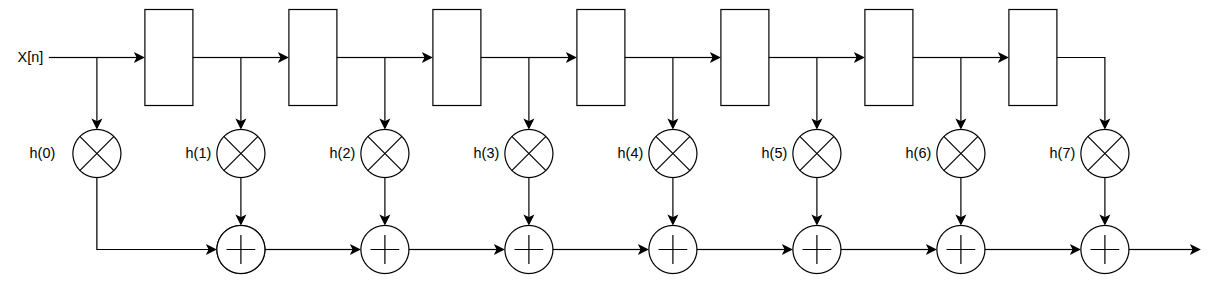
\includegraphics[width=\linewidth]{fir.png}
    \caption{Estructura de un filtro FIR genérico de ocho taps.}
    \label{fig:fir-generico}
\end{figure}

\subsection{Paralelización del filtro}

La salida de un filtro FIR de $N$ taps se expresa como:

\begin{equation}
    y[n]=\sum_{k=0}^{N-1}h_k\,x[n-k].
    \label{eq:fir-convolucion}
\end{equation}

Para obtener cuatro resultados por ciclo se escribieron explícitamente las
ecuaciones temporales del filtro, agrupando las entradas y salidas de a cuatro. A
continuación se muestra el procedimiento para el ejemplo de ocho taps de la
Figura~\ref{fig:fir-generico}. En el primer ciclo ingresan $x_0$, $x_1$, $x_2$ y
$x_3$, y las salidas correspondientes son:

\begingroup
\small
\begin{align*}
y_0={}&x_0h_0+x_{-1}h_1+x_{-2}h_2+x_{-3}h_3
       +x_{-4}h_4+x_{-5}h_5+x_{-6}h_6+x_{-7}h_7\\
y_1={}&x_1h_0+x_0h_1+x_{-1}h_2+x_{-2}h_3
       +x_{-3}h_4+x_{-4}h_5+x_{-5}h_6+x_{-6}h_7\\
y_2={}&x_2h_0+x_1h_1+x_0h_2+x_{-1}h_3
       +x_{-2}h_4+x_{-3}h_5+x_{-4}h_6+x_{-5}h_7\\
y_3={}&x_3h_0+x_2h_1+x_1h_2+x_0h_3
       +x_{-1}h_4+x_{-2}h_5+x_{-3}h_6+x_{-4}h_7
\end{align*}
\endgroup

Durante el segundo ciclo ingresan $x_4$, $x_5$, $x_6$ y $x_7$. Las cuatro nuevas
salidas combinan esas muestras con las entradas almacenadas del ciclo anterior:

\begingroup
\small
\begin{align*}
y_4={}&x_4h_0+x_3h_1+x_2h_2+x_1h_3
       +x_0h_4+x_{-1}h_5+x_{-2}h_6+x_{-3}h_7\\
y_5={}&x_5h_0+x_4h_1+x_3h_2+x_2h_3
       +x_1h_4+x_0h_5+x_{-1}h_6+x_{-2}h_7\\
y_6={}&x_6h_0+x_5h_1+x_4h_2+x_3h_3
       +x_2h_4+x_1h_5+x_0h_6+x_{-1}h_7\\
y_7={}&x_7h_0+x_6h_1+x_5h_2+x_4h_3
       +x_3h_4+x_2h_5+x_1h_6+x_0h_7
\end{align*}
\endgroup

En el tercer ciclo, las primeras cuatro entradas ya se desplazaron por la memoria
del filtro. Las ecuaciones resultan:

\begingroup
\small
\begin{align*}
y_8={}&x_8h_0+x_7h_1+x_6h_2+x_5h_3
       +x_4h_4+x_3h_5+x_2h_6+x_1h_7\\
y_9={}&x_9h_0+x_8h_1+x_7h_2+x_6h_3
       +x_5h_4+x_4h_5+x_3h_6+x_2h_7\\
y_{10}={}&x_{10}h_0+x_9h_1+x_8h_2+x_7h_3
          +x_6h_4+x_5h_5+x_4h_6+x_3h_7\\
y_{11}={}&x_{11}h_0+x_{10}h_1+x_9h_2+x_8h_3
          +x_7h_4+x_6h_5+x_5h_6+x_4h_7
\end{align*}
\endgroup

Al comparar las ecuaciones puede observarse que cada salida necesita una ventana de
ocho muestras consecutivas, pero el punto inicial de esa ventana cambia para cada
lane. Las muestras más recientes provienen directamente de las cuatro entradas del
ciclo actual y las restantes deben recuperarse de la memoria del filtro. Una vez
identificado este patrón, la construcción puede extenderse a cualquier cantidad de
taps y a sucesivos grupos de cuatro entradas.

La Figura~\ref{fig:fir-paralelo-generico} muestra el resultado de aplicar este
razonamiento al FIR genérico de ocho taps. Se obtienen cuatro caminos de suma de
productos, uno para cada salida, alimentados por las entradas actuales y por las
muestras conservadas en el regresor.

\begin{figure}[htbp]
    \centering
    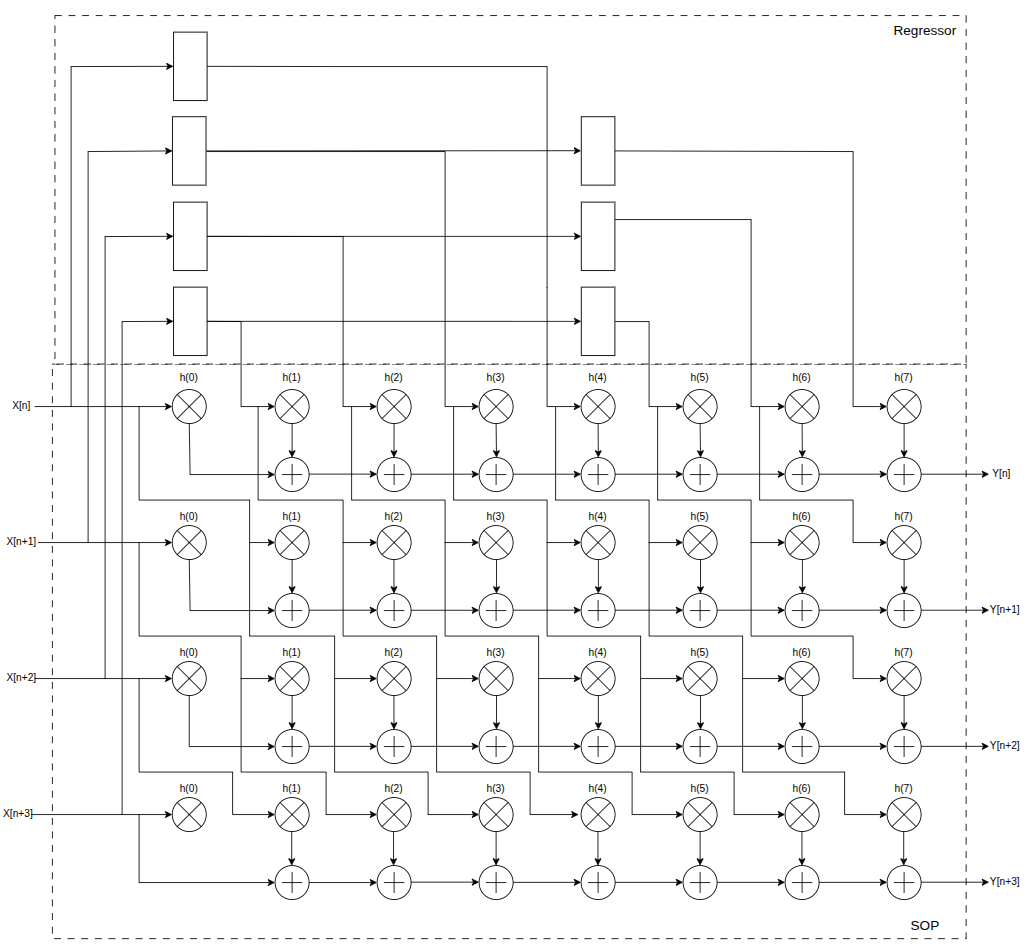
\includegraphics[width=0.92\linewidth]{../../fir_parallel/pics/rtl.png}
    \caption{Paralelización por cuatro del FIR genérico de ocho taps.}
    \label{fig:fir-paralelo-generico}
\end{figure}

\subsection{Implementación RTL}

El submódulo \texttt{regressor} conserva la historia necesaria para construir las
cuatro ventanas de convolución. En lugar de utilizar una única cadena que se desplaza
una muestra por ciclo, se implementan cuatro cadenas de registros paralelas, una por
lane de entrada. Cada nuevo ciclo desplaza simultáneamente cuatro muestras dentro de
la memoria.

Para un filtro de $N$ taps se requieren $N-1$ muestras anteriores. El número de
niveles del regresor se calcula como

\begin{equation}
    L=\left\lceil\frac{N-1}{P}\right\rceil.
    \label{eq:fir-niveles-regresor}
\end{equation}

En el diseño utilizado, $N=19$ y $P=4$, por lo que deben almacenarse 18 muestras en
cinco niveles de registros. Los primeros cuatro registros reciben las entradas del
ciclo en orden temporal inverso, de la más reciente a la más antigua. En cada nivel
siguiente se guarda el grupo proveniente del nivel anterior.

El módulo \texttt{fir\_parallel} combina esta memoria con las entradas actuales para
formar el array de muestras que será el input del modulo \texttt{sop} para cada lane.
De esta manera se obtienen cuatro resultados consecutivos por ciclo.

\subsection{Verificación}

La verificación del filtro FIR paralelo se realizó utilizando un testbench básico.
En el mismo se le ingresa una señal PAM-2 aleatoria y se comprueba su salida haciendo 
vector matching con una señal obtenida del golden reference en diseñado en python.

\clearpage

% ---------------------------------------------------------------------------
\section{Bloque C: Unidad de diagnóstico (\texttt{du})}
\label{sec:du}
% ---------------------------------------------------------------------------

\subsection{Objetivo y especificaciones}

La unidad de diagnóstico (DU) funciona como un osciloscopio digital integrado en el
sistema. Su objetivo es almacenar una ventana temporal de la señal de salida del
filtro FIR alrededor de un evento de disparo. En el top se instancian cuatro DUs, 
una por cada lane del datapath, todas controladas por la misma señal de ARM y por 
un trigger común.

Cada instancia posee una memoria de 256 palabras de 12 bits. El trigger se genera
cuando al menos una de las cuatro salidas del FIR supera el umbral configurado, 
quedando la posición del evento de disparo dentro de la ventana depende del modo 
seleccionado.

Los modos de captura de la DU se resuemen en la Tabla~\ref{tab:du-modos}.

\begin{table}[H]
    \centering
    \caption{Modos de captura de la DU. (W = 256)}
    \label{tab:du-modos}
    \begin{tabular}{ccl}
        \toprule
        \textbf{Valor} & \textbf{Modo} & \textbf{Comportamiento} \\
        \midrule
        \texttt{00} & PRE  & Captura W muestras continuamente y finaliza al recibir el trigger \\
        \texttt{01} & MID  & Conserva W/2 muestras anteriores y W/2 posteriores al trigger \\
        \texttt{10} & POST & Comienza la captura de W muestras al recibir el trigger. \\
        \bottomrule
    \end{tabular}
\end{table}

En modo PRE la memoria funciona como un buffer circular desde el ARM, capturando continuamente
hasta el evento de trigger. En modo MID también se escribe como un buffer circular antes del 
trigger, pero luego del trigger la captura continúa hasta completar media memoria más.
Para una profundidad de 256 posiciones, la ventana queda formada por 128 muestras anteriores 
y 128 posteriores al trigger. En modo POST no se escribe antes del evento sino que la muestra 
que produce el trigger es la primera de la ventana y luego se completa el resto de la memoria.

El modo se captura junto con el pulso de ARM. Si se recibe el valor reservado
\texttt{11}, el módulo selecciona MID como modo seguro por defecto.

\subsection{Arquitectura e implementación RTL}

La arquitectura de la DU se basa en una maquina de estados que controla la adquisición
de muestras y su escritura en memoria, en función del modo de captura. Esto naturalmente
se realiza en el dominio de DSP, mientras que la lectura de la memoria se realiza en el
dominio de CPU una vez la captura finalizó.

\subsubsection*{Máquina de estados}

La máquina de estados posee los estados \texttt{IDLE}, \texttt{RUN},
\texttt{CAPTURING} y \texttt{DONE}. Su funcionamiento se muestra en la
Figura~\ref{fig:du-fsm}.

\begin{figure}[H]
    \centering
    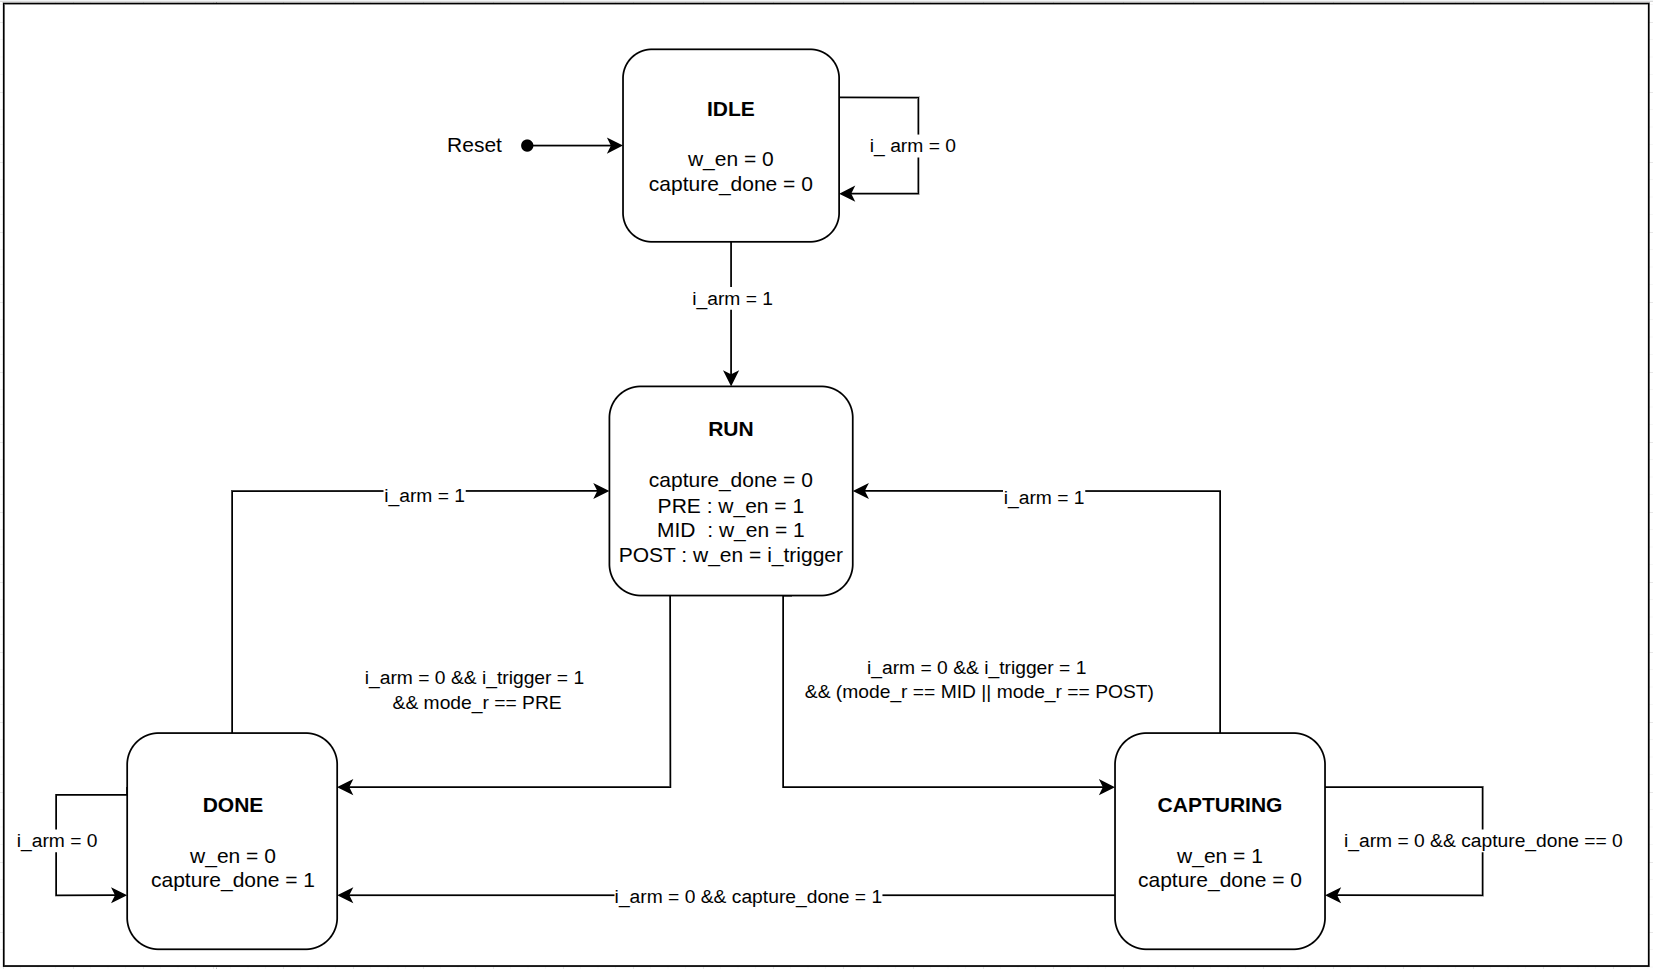
\includegraphics[width=\linewidth]{du_fsm.png}
    \caption{Máquina de estados de la DU.}
    \label{fig:du-fsm}
\end{figure}

Las ecuaciones de control de la máquina de estados se expresan a continuación:

\begin{equation}
\text{\texttt{w\_en}}=
\begin{cases}
\text{\texttt{state\_r == RUN}},
    & \text{modo PRE},\\
\text{\texttt{(state\_r == RUN) || (state\_r == CAPTURING)}},
    & \text{modo MID},\\
\text{\texttt{((state\_r == RUN) \&\& i\_trigger) || (state\_r == CAPTURING)}},
    & \text{modo POST}
\end{cases}
\label{eq:du-write-enable}
\end{equation}

El valor objetivo del contador posterior al trigger se determina mediante

\begin{equation}
\text{\texttt{target = (mode\_r == MID) ? ((DEPTH/2) - 1) : (DEPTH - 1)}}
\label{eq:du-target}
\end{equation}

Por lo tanto, la condición que finaliza la etapa de captura y la indicación interna
de captura completa son

\begin{align}
\text{\texttt{capture\_done}} & =
    \text{\texttt{(state\_r == CAPTURING) \&\& (post\_tr\_cnt\_r == target)}},
    \label{eq:du-capture-done}\\
\text{\texttt{done\_wr}} & = \text{\texttt{(state\_r == DONE)}}
    \label{eq:du-done-write}
\end{align}

En PRE no se utiliza el contador posterior al trigger porque la máquina pasa
directamente de \texttt{RUN} a \texttt{DONE}.

\subsubsection*{Escritura y lectura de memoria}

La organización de la memoria se muestra en la Figura~\ref{fig:du-memoria}. La
escritura es síncrona al clock DSP y se realiza cuando $w_{en}=1$. Durante un nuevo
ARM la escritura se frena para que el puntero y la FSM regresen a su estado inicial. 

\begin{equation}
\text{\texttt{mem[ptr\_wr] <= i\_data}}
\quad\text{si}\quad
\text{\texttt{w\_en \&\& !i\_arm}}
\label{eq:du-memory-write}
\end{equation}

El puntero \texttt{ptr\_wr} se incrementa con cada escritura, utilizando un contador
que hace overflow al llegar al tamaño de la memoria. Cuando la memoria está completa, 
el puntero indica la dirección de la muestra más antigua, permitiendo reconstruir la 
captura en orden cronológico.

\begin{figure}[H]
    \centering
    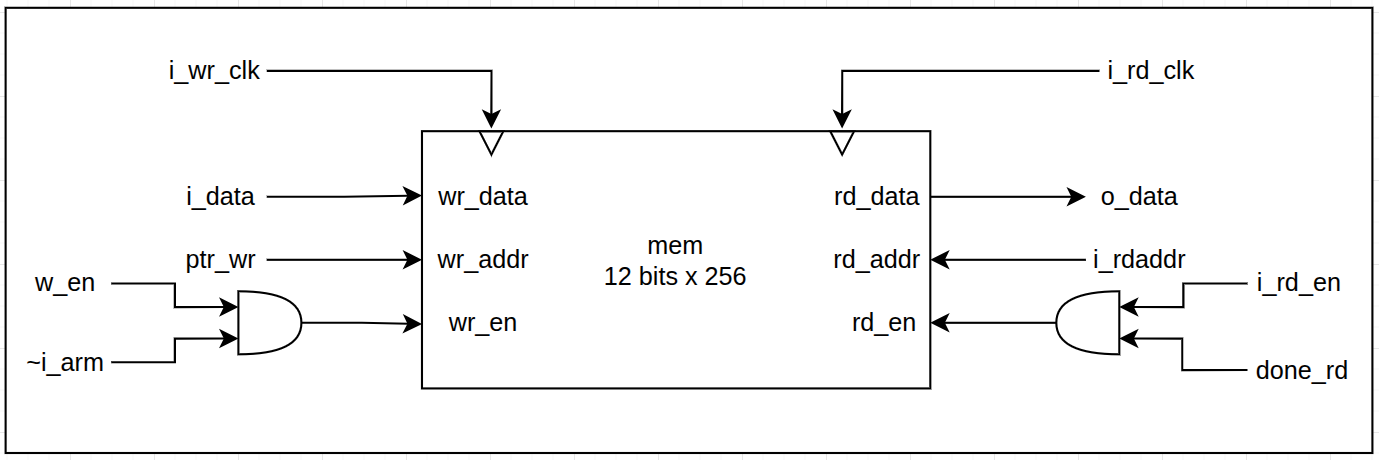
\includegraphics[width=0.9\linewidth]{du_mem.png}
    \caption{Organización de los puertos de escritura y lectura de la memoria de la DU.}
    \label{fig:du-memoria}
\end{figure}

La señal \texttt{done\_wr} se sincroniza hacia el dominio CPU, con un sincronizador 
de FF. La lectura solo se habilita cuando esta señal sincronizada está activa, 
evitando accesos mientras la memoria aún está siendo modificada. El puerto de lectura 
es síncrono: ante \texttt{i\_rd\_en} y una dirección válida, el dato se registra en
\texttt{o\_data} y \texttt{o\_rd\_valid} se activa durante la respuesta. El puntero
final también se mantiene estable y se entrega al mapa de registros para que el
software determine la primera dirección que debe leer.

\subsection{Verificación}

La DU se verificó mediante un testbench con clocks independientes para los dominios
DSP y CPU. Se aplicó como entrada una secuencia PRBS conocida y se ejecutó una
adquisición completa en cada uno de los modos PRE, MID y POST. Para cada caso se armó
la DU, se generó el trigger, se esperó al flag de done y se leyó la memoria completa 
desde la posición informada por el puntero. Las 256 muestras recuperadas se compararon 
con las posiciones esperadas de la secuencia de referencia, comprobando tanto la 
ubicación temporal del trigger como el orden de lectura y el funcionamiento del buffer
circular.

% ---------------------------------------------------------------------------
\section{Bloque D: Medidor de frecuencia (\texttt{freq\_meas})}
\label{sec:freq-meas}
% ---------------------------------------------------------------------------

\subsection{Objetivo}

El medidor de frecuencia permite determinar la frecuencia de un clock desconocido a
partir de otro clock cuya frecuencia es conocida. En este sistema se utiliza el clock
de CPU de 200 MHz como referencia para medir el clock DSP, cuya frecuencia es
1 GHz. Aunque este bloque no forma parte del datapath, permite comprobar desde 
software que ambos clocks están funcionando correctamente.

\subsection{Principio de funcionamiento}

El principio de medición consiste en generar, dentro del dominio de referencia, una
ventana con una duración conocida. Mientras la ventana está activa se cuentan los
flancos ascendentes del clock a medir. Si la ventana permanece activa durante
$W$ ciclos del clock de referencia, su duración es:

\begin{equation}
    T_W=\frac{W}{f_{ref}}
    \label{eq:freq-window-time}
\end{equation}

Si durante ese intervalo se cuentan $N_{in}$ ciclos del clock desconocido, su
frecuencia puede estimarse como:

\begin{equation}
    \widehat{f}_{in}=\frac{N_{in}}{T_W}
    =\frac{N_{in}\,f_{ref}}{W}
    \label{eq:freq-estimation}
\end{equation}

Para $f_{ref}=200\ \text{MHz}$ y una frecuencia de entrada nominal de
$f_{in}=1\ \text{GHz}$, la cantidad esperada de ciclos dentro de la ventana es

\begin{equation}
    N_{in}=W\frac{f_{in}}{f_{ref}}=5W
    \label{eq:freq-expected-count}
\end{equation}


Como el resultado se obtiene contando flancos, la mínima variación es de
una cuenta. Esa variación equivale a un paso de frecuencia
$\Delta f=f_{ref}/W$. La resolución relativa compara dicho paso con la frecuencia
medida y expresa qué fracción del valor total representa la menor diferencia que el
frecuencímetro puede distinguir. Cuanto menor es esta relación, mayor es la precisión
de la medición; por ejemplo, una resolución de 1 ppm equivale a una parte en un
millón, es decir, $10^{-6}$. Por lo tanto, la resolución relativa del contador es:

\begin{equation}
    \frac{\Delta f}{f_{in}} =\frac{f_{ref}}{W\,f_{in}}
    =\frac{1}{N_{in}}
    \label{eq:freq_resolution}
\end{equation}

Para obtener un error de 1ppm ($10^{-6}$) se requiere entonces:

\begin{equation}
    \frac{1}{5W}< 10^{-6}
    \quad\Longrightarrow\quad
    W>200000
    \label{eq:freq-min-window}
\end{equation}

Por lo que se eligió $W=200\,000$ como valor de ventana. A 200 MHz esto corresponde 
a una ventana de 1 ms, dentro de la cual se esperan:

\begin{equation}
    N_{in}=5\cdot 200\,000=1\,000\,000
    \label{eq:freq-count-nominal}
\end{equation}

ciclos del clock DSP.

El ancho mínimo de cada contador se obtiene calculando la cantidad de bits necesaria
para representar su máximo valor:

\begin{align}
    B_W & = \left\lceil\log_2(W+1)\right\rceil
          = \left\lceil\log_2(200\,001)\right\rceil = 18,
          \label{eq:freq-window-width}\\
    B_C & = \left\lceil\log_2(N_{in}+1)\right\rceil
          = \left\lceil\log_2(1\,000\,001)\right\rceil = 20.
          \label{eq:freq-count-width}
\end{align}

El RTL utiliza \texttt{WIN\_W=19}, incorporando un bit de margen para la longitud
programable de la ventana, y \texttt{CNT\_W=20} para el contador del clock de entrada.
Con una cuenta nominal de un millón, este último permanece por debajo de su máximo
valor representable, $2^{20}-1=1\,048\,575$.

\subsection{Arquitectura e implementación RTL}

La arquitectura del frecuencímetro se muestra en la
Figura~\ref{fig:freq-meas-rtl}. El dominio de referencia contiene el registro de
configuración de la ventana, el contador de ciclos de CPU y la lógica que genera el
nivel \texttt{window\_open\_ref\_r}. Ante un pulso de \texttt{i\_start}, el módulo
captura \texttt{i\_window\_len}, reinicia el contador y abre una nueva ventana. El
nivel permanece activo hasta que transcurre la cantidad de ciclos programada.

\begin{figure}[H]
    \centering
    
\includegraphics[width=\linewidth]{../../freq_meas/pics/rtl.png}
    \caption{Arquitectura RTL del medidor de frecuencia.}
    \label{fig:freq-meas-rtl}
\end{figure}

La ventana se sincroniza hacia el dominio del clock de entrada. Allí, un detector de
flanco ascendente genera el pulso que limpia el resultado anterior y un detector de
flanco descendente identifica el final de la medición. Mientras el nivel sincronizado
permanece activo, \texttt{input\_cnt\_r} se incrementa con cada flanco de
\texttt{i\_clk\_in}. Al cerrarse la ventana, el contador queda congelado y se activa
la indicación \texttt{done\_in\_r}.

Un nuevo pulso de \texttt{i\_start} invalida inmediatamente el resultado previo. Además, 
la longitud de ventana se captura al comenzar la medición, por lo que una modificación
posterior de \texttt{i\_window\_len} no afecta la cuenta en curso.

\subsection{Cruces de dominio de clock}

El diseño tiene dos cruces de dominio implementados mediante sincronizadores de
FF. El primero transfiere el nivel \texttt{window\_open\_ref\_r} desde el
dominio de referencia hacia el dominio de entrada. Como la ventana permanece activa
durante una gran cantidad de ciclos, el nivel puede atravesar el sincronizador sin
problema. Los detectores de flanco generan luego pulsos de un ciclo ya
síncronos a \texttt{i\_clk\_in}.

El segundo cruce transfiere el nivel \texttt{done\_in\_r} en sentido contrario. Esta 
señal se mantiene en uno desde que finaliza una medición hasta que comienza la siguiente, 
por lo que también puede sincronizarse como nivel sin problema.

El contador \texttt{input\_cnt\_r} es un bus de múltiples bits y no se sincroniza bit
a bit, sino que se utiliza una transferencia de tipo bundled-data. Cuando 
\texttt{done\_in\_r} se activa, el contador deja de modificarse y permanece estable
hasta el proximo inicio. De esta manera, \texttt{o\_done} funciona como flag de validez 
de \texttt{o\_count}. La latencia del sincronizador dá  varios ciclos para que el dato 
se estabilice antes de ser observado desde el dominio CPU.

\subsection{Medición de un clock de 8 GHz}

Para conservar una resolución relativa de 1 ppm es necesario observar, como mínimo un 
millón de ciclos del clock a medir. A partir de la Ecuación~\ref{eq:freq-expected-count}, 
la longitud de ventana requerida para una frecuencia cualquiera puede calcularse como

\begin{equation}
    W_{1\,\mathrm{ppm}}
    =\left\lceil 10^6\frac{f_{ref}}{f_{in}}\right\rceil.
    \label{eq:freq-window-one-ppm}
\end{equation}

Para el caso de 8GHz planteado a en la consigna, utilizando un clock
de 200 MHz se requieren

\begin{equation}
    W_{8\,\mathrm{GHz}}
    =10^6\frac{200\,\mathrm{MHz}}{8\,\mathrm{GHz}}
    =25\,000,
    \label{eq:freq-window-8ghz}
\end{equation}

equivalente a 125 $\mu$s. Por lo tanto, desde el punto de vista de los anchos de los
contadores, el clock de 8 GHz puede medirse sin modificaciones: la ventana de 25 000
ciclos entra en \texttt{WIN\_W=19} y el resultado continúa siendo de aproximadamente
un millón de cuentas, por debajo del máximo de \texttt{CNT\_W=20}.

Sin embargo, es posible que la limitación sea de timing, ya que el contador debe 
poder operar físicamente a 8 GHz. Si el circuito no cierra timing a esa frecuencia, 
el método es matemáticamente válido pero la implementación no.

Son las frecuencias bajas las que exigen ventanas más largas para acumular el millón 
de cuentas necesario. Con \texttt{WIN\_W=19}, la máxima ventana programable es de 
$2^{19}-1=524\,287$ ciclos, o aproximadamente 2.62 ms a 200 MHz. Por lo tanto,
la menor frecuencia para la cual puede alcanzarse una resolución de 1 ppm con los
anchos actuales es aproximadamente

\begin{equation}
    f_{in,\min}
    =\frac{10^6\,f_{ref}}{2^{19}-1}
    \approx 381.5\ \mathrm{MHz}.
    \label{eq:freq-min-one-ppm}
\end{equation}

Es decir, oueden medirse clocks más lentos, pero con una resolución relativa peor 
que 1 ppm.

\subsection{Verificación}

La verificación se realizó con clocks de 200 MHz y 1 GHz y una ventana de 200 000
ciclos de referencia. Se comprobó que la cuenta obtenida estuviera en el rango
cercano de 1 000 000 ciclos y que \texttt{o\_count} permaneciera estable mientras
\texttt{o\_done} estuviera activo. También se inició una segunda medición para
verificar que \texttt{i\_start} invalidara el resultado anterior y que un cambio de
\texttt{i\_window\_len} durante la medición no modificara la ventana ya capturada.

El resultado obtenido fue el error de una cuenta, es decir 999 999.

% ---------------------------------------------------------------------------
\section{Bloque E: Mapa de registros (\texttt{regmap})}
\label{sec:regmap}
% ---------------------------------------------------------------------------

\subsection{Objetivo}

El mapa de registros es la interfaz entre el software y los distintos
bloques de hardware del sistema. Su función es centralizar la configuración y el
control de los módulos, permitiendo también la lectura de sus resultados y señales
de estado. Para ello, decodifica las direcciones recibidas desde la CPU y las
traduce en registros de configuración, pulsos de control o accesos a información
generada por el hardware.

\subsection{Arquitectura e interfaz}

El bloque funciona de manera sincrónica al clock de CPU y presenta una interfaz
simple formada por el address del registro texttt{i\_addr}, dato de escritura
\texttt{i\_wdata}, request \texttt{i\_req} y tipo de operación
\texttt{i\_is\_write}. Como respuesta, entrega el dato de lectura
\texttt{o\_rdata} y la confirmación \texttt{o\_ack}.

Internamente, la dirección selecciona el registro involucrado en la transacción.
Los campos de configuración se almacenan en registros, mientras que los campos de
estado se obtienen directamente de los módulos correspondientes.

La Figura~\ref{fig:regmap-rtl} muestra un esquema simplificado de la arquitectura.
El dato de escritura se dirige al banco de registros seleccionado por
\texttt{i\_addr}; para las lecturas, un multiplexor selecciona el valor que será
registrado en \texttt{o\_rdata}. La señal \texttt{o\_ack} indica que la
transacción fue atendida, en ambos casos por igual.

\begin{figure}[H]
    \centering
    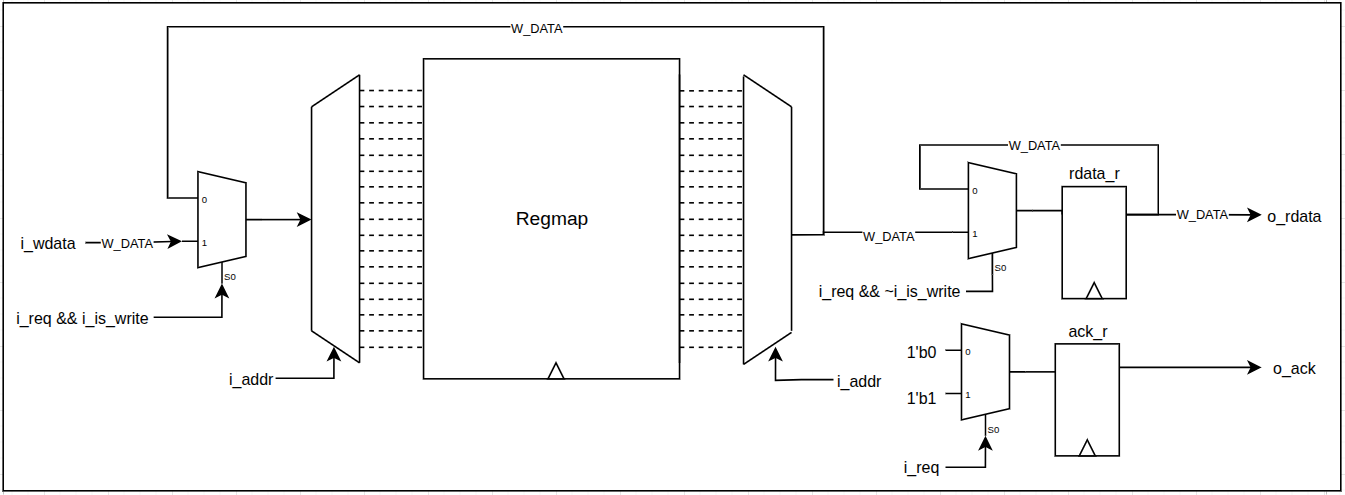
\includegraphics[width=\linewidth]{regmap_rtl.png}
    \caption{Arquitectura RTL simplificada del mapa de registros.}
    \label{fig:regmap-rtl}
\end{figure}

\subsection{Transacciones de acceso}

\subsubsection*{Escritura}
Para realizar una escritura, el SW coloca la dirección y el dato sobre
\texttt{i\_addr} e \texttt{i\_wdata}, respectivamente, y activa simultáneamente
\texttt{i\_req} e \texttt{i\_is\_write}. En el proximo flanco positivo del clock, 
el \texttt{regmap} decodifica la dirección y actualiza el registro correspondiente.
La aceptación de la operación se informa mediante un pulso en \texttt{o\_ack}, un 
ciclo de clock despues del request.

\subsubsection*{Lectura}

En una lectura, el SW coloca la dirección y activa \texttt{i\_req},
manteniendo \texttt{i\_is\_write} en bajo. EEl bloque decodifica la dirección, y al 
proximo flanco positivo del clock escribe el valor seleccionado en \texttt{o\_rdata} 
y activa \texttt{o\_ack} para indicar que el dato es válido. 
Las direcciones no implementadas devuelven cero.

La Figura~\ref{fig:regmap-transacciones} muestra las formas de onda de ambas
operaciones. En los dos casos, la dirección y las señales de control se presentan
antes del flanco de captura, mientras que la confirmación se observa un ciclo
después.

\begin{figure}[H]
    \centering
    \begin{minipage}[t]{0.48\linewidth}
        \centering
        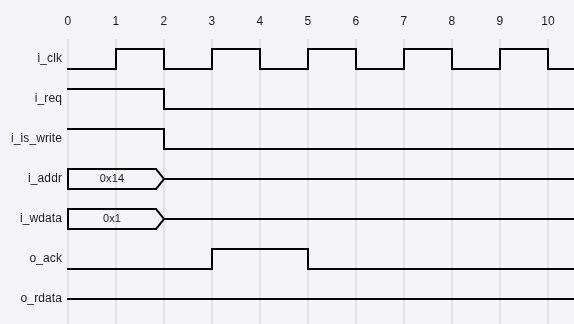
\includegraphics[width=\linewidth]{write_seq.png}
        \smallskip

        \small (a) Secuencia de escritura.
    \end{minipage}
    \hfill
    \begin{minipage}[t]{0.48\linewidth}
        \centering
        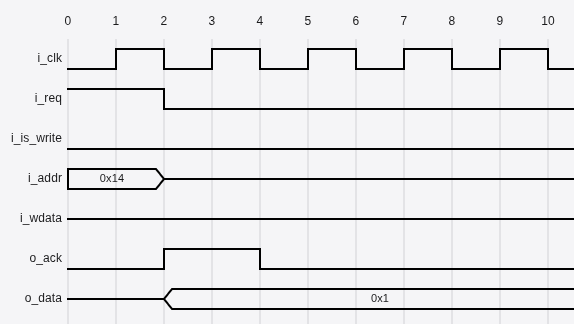
\includegraphics[width=\linewidth]{read_seq.png}
        \smallskip

        \small (b) Secuencia de lectura.
    \end{minipage}
    \caption{Transacciones de acceso al mapa de registros.}
    \label{fig:regmap-transacciones}
\end{figure}

La lectura de \texttt{DU\_RDDATA} constituye un caso particular, debido a la latencia 
de la memoria de la DU. Cuando las cuatro unidades finalizaron la captura, el acceso 
genera el pedido de lectura y mantiene la transacción pendiente hasta recibir 
\texttt{i\_du\_rd\_valid}. Recién entonces se entrega el dato y se activa 
\texttt{o\_ack}. Si las DUs todavía no finalizaron, la lectura devuelve cero sin 
iniciar el acceso a memoria.

\subsection{Mapa de direcciones}
\label{subsec:mapa-direcciones}

La Tabla~\ref{tab:regmap} resume los registros accesibles por software y su
interacción con el hardware.

\begin{longtable}{@{}
    >{\centering\arraybackslash}p{0.08\textwidth}
    >{\raggedright\arraybackslash}p{0.19\textwidth}
    >{\centering\arraybackslash}p{0.06\textwidth}
    >{\centering\arraybackslash}p{0.06\textwidth}
    >{\raggedright\arraybackslash}p{0.49\textwidth}@{}
}

\caption{Mapa de registros del sistema.}
\label{tab:regmap}\\

\toprule
\textbf{Addr} &
\textbf{Registro} &
\textbf{SW} &
\textbf{HW} &
\textbf{Descripción} \\
\midrule
\endfirsthead

\toprule
\textbf{Addr} &
\textbf{Registro} &
\textbf{SW} &
\textbf{HW} &
\textbf{Descripción} \\
\midrule
\endhead

\midrule
\multicolumn{5}{r}{Continúa en la página siguiente.} \\
\endfoot

\bottomrule
\endlastfoot

% ---------------------------------------------------------------------------
% PRBS
% ---------------------------------------------------------------------------

\texttt{0x00} &
\texttt{PRBS\_CTRL} &
R/W &
R &
\texttt{bit[0]} = START, inicio de secuencia

\texttt{bit[1]} = STOP, detención de secuencia

\texttt{bit[4:2]} = SEL, selección de PRBS10-15 \\


\texttt{0x01} &
\texttt{PRBS\_SEED} &
R/W &
R &
\texttt{bit[14:0]} = SEED inicial del LFSR \\


\texttt{0x02} &
\texttt{PRBS\_STATUS} &
R &
W &
\texttt{bit[0]} = RUNNING, secuencia activa\\


% ---------------------------------------------------------------------------
% FIR
% ---------------------------------------------------------------------------

\texttt{0x10} &
\texttt{FIR\_TAP\_0} &
R/W &
R &
\texttt{bit[11:0]} = coeficiente FIR $h_0$, S(12,10) \\

\texttt{0x11} &
\texttt{FIR\_TAP\_1} &
R/W &
R &
\texttt{bit[11:0]} = coeficiente FIR $h_1$, S(12,10) \\

\texttt{0x12} &
\texttt{FIR\_TAP\_2} &
R/W &
R &
\texttt{bit[11:0]} = coeficiente FIR $h_2$, S(12,10) \\

\texttt{0x13} &
\texttt{FIR\_TAP\_3} &
R/W &
R &
\texttt{bit[11:0]} = coeficiente FIR $h_3$, S(12,10) \\

\texttt{0x14} &
\texttt{FIR\_TAP\_4} &
R/W &
R &
\texttt{bit[11:0]} = coeficiente FIR $h_4$, S(12,10) \\

\texttt{0x15} &
\texttt{FIR\_TAP\_5} &
R/W &
R &
\texttt{bit[11:0]} = coeficiente FIR $h_5$, S(12,10) \\

\texttt{0x16} &
\texttt{FIR\_TAP\_6} &
R/W &
R &
\texttt{bit[11:0]} = coeficiente FIR $h_6$, S(12,10) \\

\texttt{0x17} &
\texttt{FIR\_TAP\_7} &
R/W &
R &
\texttt{bit[11:0]} = coeficiente FIR $h_7$, S(12,10) \\

\texttt{0x18} &
\texttt{FIR\_TAP\_8} &
R/W &
R &
\texttt{bit[11:0]} = coeficiente FIR $h_8$, S(12,10) \\

\texttt{0x19} &
\texttt{FIR\_TAP\_9} &
R/W &
R &
\texttt{bit[11:0]} = coeficiente FIR $h_9$, S(12,10) \\


\texttt{0x1A} &
\texttt{FIR\_CTRL} &
R/W &
R &
\texttt{bit[0]} = COMMIT, transferir los coeficientes al filtro

\texttt{bit[1]} = ENABLE del filtro \\


\texttt{0x1B} &
\texttt{FIR\_STATUS} &
R &
W &
\texttt{bit[0]} = BUSY
Vale uno mientras se encuentra en curso la transferencia de coeficientes.
Los coeficientes deben permanecer estables durante este intervalo. \\

% ---------------------------------------------------------------------------
% Data Unit
% ---------------------------------------------------------------------------

\texttt{0x20} &
\texttt{DU\_CTRL} &
R/W &
R &
\texttt{bit[0]} = ARM, inicia o reinicia la adquisición

\texttt{bit[2:1]} = MODE: PRE, MID y POST \\

\texttt{0x21} &
\texttt{DU\_THRESHOLD} &
R/W &
R &
\texttt{bit[11:0]} = umbral de disparo, S(12,10) \\

\texttt{0x22} &
\texttt{DU\_STATUS} &
R &
W &
\texttt{bit[3:0]} = DONE.
bit 0 = DU0, bit 1 = DU1, bit 2 = DU2 y bit 3 = DU3 \\

\texttt{0x23} &
\texttt{DU\_RDADDR} &
R/W &
R &
\texttt{bit[7:0]} = dirección de lectura de la DU seleccionada \\

\texttt{0x24} &
\texttt{DU\_RDDATA} &
R &
W &
\texttt{bit[11:0]} = muestra leída de la DU seleccionada0, S(12,10) \\

\texttt{0x25} &
\texttt{DU\_RDPTR} &
R &
W &
\texttt{bit[7:0]} = posición de memoria inicial de lectura de la DU seleccionada\\

\texttt{0x26} &
\texttt{DU\_SELECT} &
R/W &
R &
\texttt{bit[1:0]} = selector de la DU utilizada para lectura.
00 = DU0, 01 = DU1, 10 = DU2 y 11 = DU3. \\

% ---------------------------------------------------------------------------
% Frequency meter
% ---------------------------------------------------------------------------

\texttt{0x30} &
\texttt{CLKMEAS\_CTRL} &
W &
R &
\texttt{bit[0]} = START, inicia nueva medición \\

\texttt{0x31} &
\texttt{CLKMEAS\_WINDOW} &
R/W &
R &
\texttt{bit[18:0]} = largo de ventana de medición en cuentas del clock de referencia CPU\\

\texttt{0x32} &
\texttt{CLKMEAS\_COUNT} &
R &
W &
\texttt{bit[19:0]} = cuentas del clock DSP durante la ventana de referencia\\

\texttt{0x33} &
\texttt{CLKMEAS\_STATUS} &
R &
W &
\texttt{bit[0]} = DONE \\

\end{longtable}

\subsection{Verificación}

La verificación se realizó mediante una prueba de configuración y lectura
utilizando el set de registros del frecuencímetro. En primer lugar, se
forzó desde el testbench un resultado de cuenta y su señal de finalización, y se
comprobó su lectura a través de \texttt{CLKMEAS\_COUNT} y
\texttt{CLKMEAS\_STATUS}. Luego se escribió un valor de ventana en
\texttt{CLKMEAS\_WINDOW}, verificando tanto su propagación hacia la salida de
configuración como su posterior lectura desde el bus.

En todos los accesos se comprobó la generación de \texttt{o\_ack}, el valor de
\texttt{o\_rdata} en las lecturas y la correcta actualización de las salidas del
frecuencímetro. De esta forma se validaron las operaciones básicas de escritura,
lectura y consulta de estado del mapa de registros.

% ---------------------------------------------------------------------------
\section{Integración del sistema (\texttt{top})}
\label{sec:top}
% ---------------------------------------------------------------------------

\subsection{Arquitectura e integración}

El módulo \texttt{top} instancia los bloques presentados en las secciones
anteriores y hace sus conexiones, con el especial cuidado de respetar los CDC. 
Como se observa en la Figura~\ref{fig:top-arquitectura}, el \texttt{regmap} 
recibe el bus externo en el dominio de CPU y distribuye la configuración hacia 
cada bloque, en su respectivo dominio de clock.

\begin{figure}[H]
    \centering
    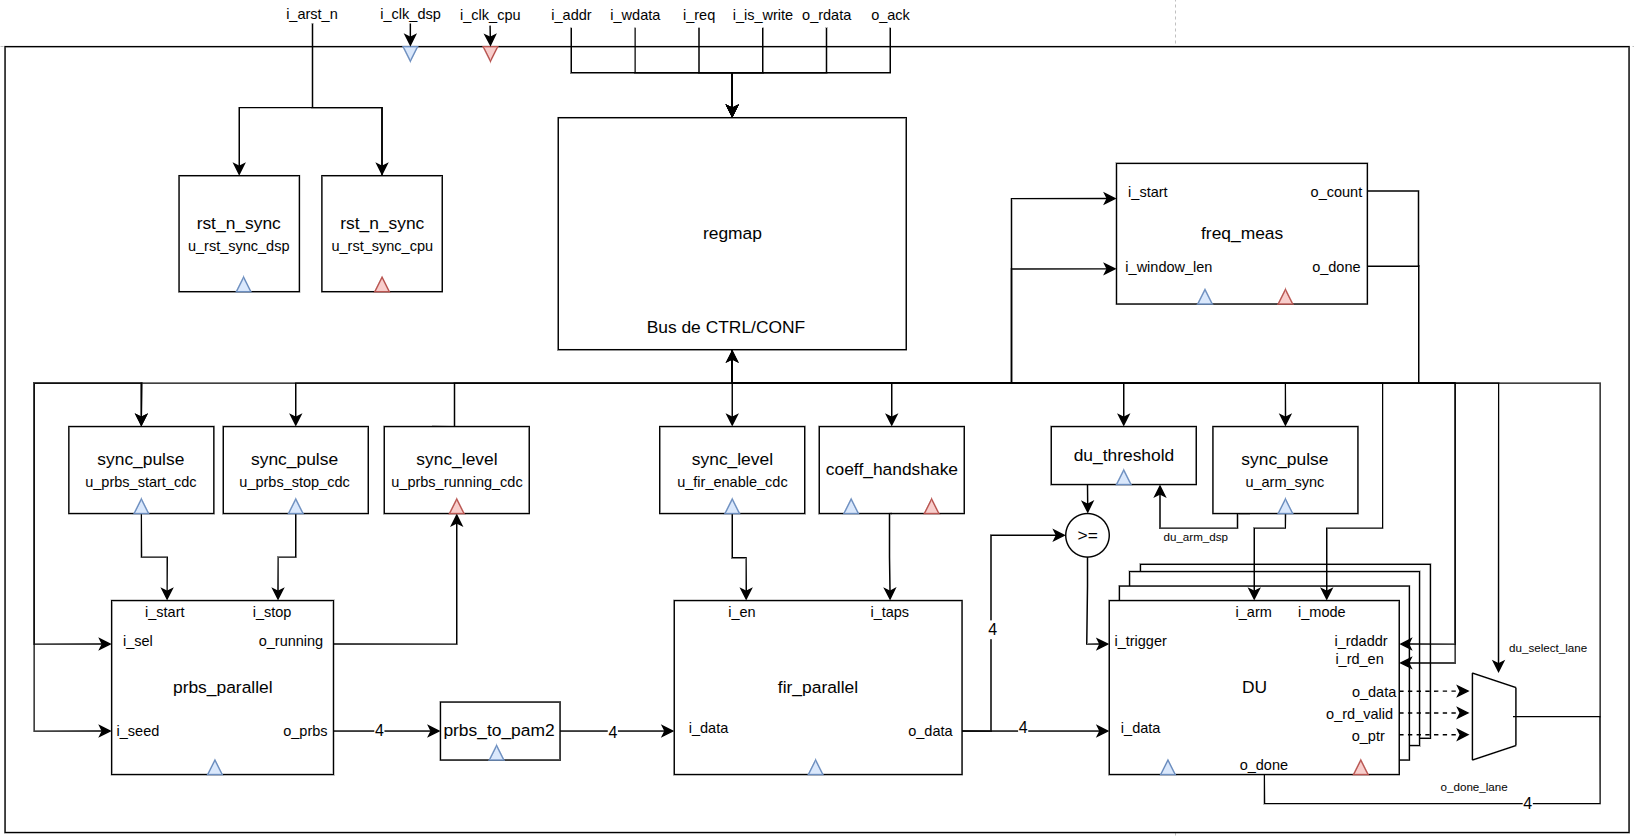
\includegraphics[width=\linewidth]{top.png}
    \caption{Interconexión de los bloques del sistema en el módulo \texttt{top}.}
    \label{fig:top-arquitectura}
\end{figure}

\subsubsection*{Reset Global}

El sistema recibe un único reset asíncrono activo en bajo, \texttt{i\_arst\_n}.
Su aserción se propaga de forma asíncrona a todo el diseño, mientras que su
liberación se sincroniza independientemente en los dominios CPU y DSP mediante
dos instancias de \texttt{rst\_n\_sync}. De esta manera, cada bloque abandona el
estado de reset sobre un flanco válido de su propio clock.

\subsubsection*{Cruces de dominio de clock}

Los pulsos \texttt{START} y \texttt{STOP} de la PRBS, y \texttt{ARM} de las
DUs, cruzan desde CPU hacia DSP mediante sincronizadores de FF con detector 
de flanco, ya que al ir de un clock lento a uno rápido se debe transferir el pulso
a la duración del clock rápido para evitar que dure mas de un ciclo de clock. 
Por otro lado, las señales de nivel \texttt{PRBS\_RUNNING} y \texttt{FIR\_ENABLE} 
utilizan sincronizadores de nivel con FF. La semilla y el selector de polinomio 
permanecen estables alrededor del pulso \texttt{START}, por lo que se transfieren 
como bundled-data y se capturan en el dominio DSP al iniciar la PRBS. De la misma 
manera, el modo y el umbral de las DUs se configuran antes de \texttt{ARM}, y se 
registran en el dominio DSP cuando llega dicho pulso.

El frecuencímetro resuelve internamente sus cruces de dominio. Pero se destaca 
que el resultado de cuenta se transfiere como bundled-data tambipén, utilizando
\texttt{o\_done} como indicación de que el dato ya se encuentra estable.

\subsubsection*{Transferencia de coeficientes del FIR}

Para cargar los coeficientes al filtro FIR, primero se deberán escribir 
los diez coeficientes independientemente en el regmap, donde se guardarán en los 
llamados registros \emph{shadow}. Una escritura del bit \texttt{COMMIT} activará la 
transacción utilizando el bloque\texttt{coeff\_handshake} y poniendo el bit 
\texttt{BUSY} en alto. Durante este periodo, no se podrá modificar el valor de los 
coeficientes en el regmap, ya que se estarán registrando en el dominio de DSP.
Una vez que se termina la transacción, se libera \texttt{BUSY} y ahora los coeficientes
cargados en los registros llamados \emph{active} serán los utilizados por el filtro FIR.

Este mecanismo implementa un cruce de bundled-data: mientras la transferencia
está en curso, los registros \emph{shadow} permanecen estables y el handshake
garantiza que el filtro actualice todos los coeficientes en el mismo evento, sin
mezclar valores pertenecientes a configuraciones diferentes.

\subsubsection*{Datapath y captura}

El bloque \texttt{prbs\_to\_pam2} convierte cada bit de la salida paralela de la
PRBS en una muestra con signo de dos bits. El bit uno se representa mediante
$+1$, mientras que el bit cero se representa mediante $-1$. Las cuatro muestras
resultantes ingresan simultáneamente al FIR paralelo.

Las cuatro salidas del FIR se comparan con un valor umbral común, que fue registrado
en el dominio de DSP al momento del armado de la DU. Si al menos una de ellas resulta 
mayor o igual que el umbral, se genera un único trigger compartido para las cuatro DUs:

\begin{equation}
    \texttt{du\_trigger\_dsp} =
    \bigvee_{i=0}^{3}
    \left(\texttt{fir\_odata\_dsp[i]} >=
    \texttt{du\_threshold\_dsp}\right).
\end{equation}

Esto permite que las cuatro lanes comiencen su captura al mismo tiempo. Para la lectura, 
\texttt{DU\_SELECT} habilita únicamente la memoria de la DU elegida mediante el regmap, 
que controla un multiplexor que devuelve al mismo su muestra, su señal \texttt{RD\_VALID} 
y su puntero final. Se optó hacerlo de esta forma para reducir tamaño de buses ya que 
podrían generar una gran congestión. En cambio, las cuatro señales \texttt{DONE} se 
conservan por separado para informar el estado completo de la captura.

\subsection{Verificación}

La verificación del sistema integrado se realizó mediante un entorno UVM basado
en clases, cuya organización se muestra en la Figura~\ref{fig:top-verificacion}. 
La secuencia genera las transacciones de configuración y lectura; el driver las 
convierte en accesos al bus del \texttt{regmap}; el monitor observa pasivamente 
las operaciones completadas; y el scoreboard comprueba que los estados y 
resultados obtenidos sean coherentes con la secuencia ejecutada. La comunicación 
entre estos componentes se implementó mediante mailboxes y una interfaz virtual.

\begin{figure}[H]
    \centering
    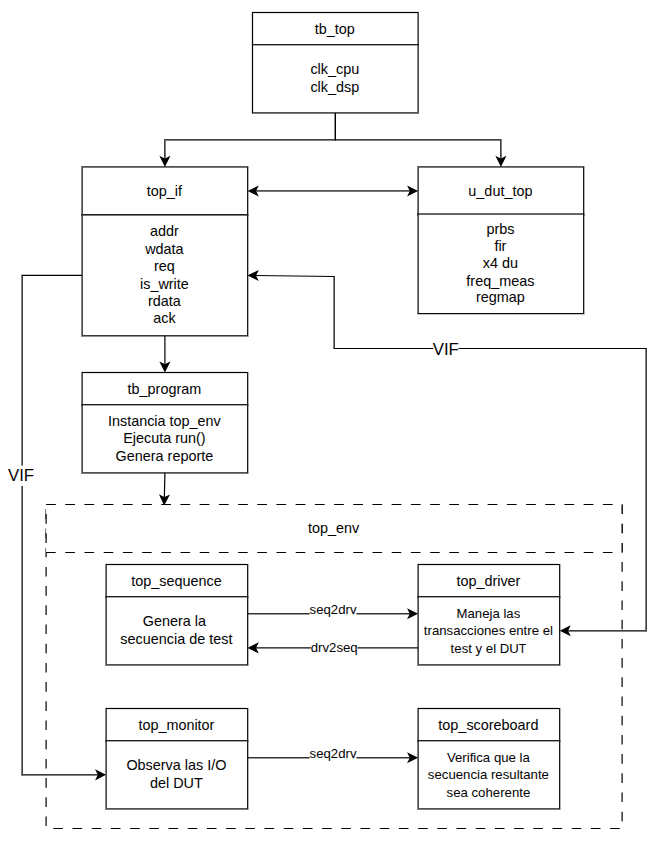
\includegraphics[width=0.62\linewidth]{uvm_top.png}
    \caption{Entorno de verificación del sistema integrado.}
    \label{fig:top-verificacion}
\end{figure}

La secuencia del test comienza aplicando el reset y configurando todos los bloques desde el
mapa de registros. Se carga una semilla \texttt{0xFFFF} y se selecciona PRBS15;
se escriben los diez coeficientes independientes del FIR y se ejecuta su
\texttt{COMMIT}, verificando la secuencia \texttt{BUSY}--\texttt{READY}. También
se configura la DU en modo POST con umbral cero y se programa la ventana del
frecuencímetro. Antes de iniciar el procesamiento, se leen nuevamente los
registros para comprobar su configuración.

En primer lugar, se hace la medición del clock de 1~GHz con el de200~MHz, y se
comprueba que el resultado esté dentro del rango deseado. Luego se inicia la
PRBS, se verifica su estado \texttt{RUNNING} en alto, se habilita el FIR y se arman las
cuatro DUs. Una vez que las cuatro indican \texttt{DONE}, se selecciona cada lane
por separado y se leen su puntero y las 256 posiciones de memoria. El scoreboard
comprueba que no existan valores desconocidos, que se hayan leído las 256 muestras
de cada DU y que las mismas no estén vacias. Para terminar, se detiene la PRBS, se verifica 
la desactivación de \texttt{RUNNING} y se deshabilita el filtro.

\subsection{Resultados de síntesis}
\label{subsec:top-sintesis}

La síntesis se evaluó a partir de cuatro métricas: timing, área, potencia y
cantidad de tipos de celdas segun tensión de umbral. Estos resultados permiten
comprobar el cumplimiento de frecuencia y reconocer qué bloques y tipos de celda
dominan el costo del diseño.

\subsubsection*{Timing}
El diseño cumple las restricciones de timing para ambos clocks, de 200~MHz y
1~GHz.

\begin{table}[H]
    \centering
    \caption{Resultado de timing del top.}
    \label{tab:top-slack}
    \begin{tabular}{@{}lll@{}}
        \toprule
        \textbf{Métrica} & \textbf{Valor} & \textbf{Unidad} \\
        \midrule
        Required time & 0.95 & ns \\
        Arrival time & -0.91 & ns \\
        \midrule
        Slack & 0.04 (MET) & ns \\
        \bottomrule
    \end{tabular}
\end{table}

El critical path pertenece al dominio del clock más rápido, de 1~GHz, y queda
identificado por los siguientes puntos:

\begin{itemize}
    \item \textbf{Startpoint:} \texttt{u\_fir\_parallel/o\_data\_reg}.
    \item \textbf{Endpoint:} \texttt{clock\_gate\_gen\_du\_lane}.
\end{itemize}

Por lo tanto, el camino crítico comienza en los registros de salida del filtro
FIR y finaliza en la lógica de clock gating, probablemente asociado a \texttt{w\_en}.

\subsubsection*{Área}

La Figura~\ref{fig:top-area} presenta la distribución del área entre los principales 
bloques. El área total obtenida fue de $21\,060\,\mu\text{m}^{2}$. Las cuatro DUs 
ocupan en conjunto $18\,600\,\mu\text{m}^{2}$, equivalentes al 88\% del total, 
debido principalmente a las memorias necesarias para almacenar las muestras. El 
FIR queda en segundo lugar, con $1\,600\,\mu\text{m}^{2}$, mientras que el resto
proviene del PRBS, el frecuencímetro, regmap y otros.

\begin{figure}[H]
    \centering
    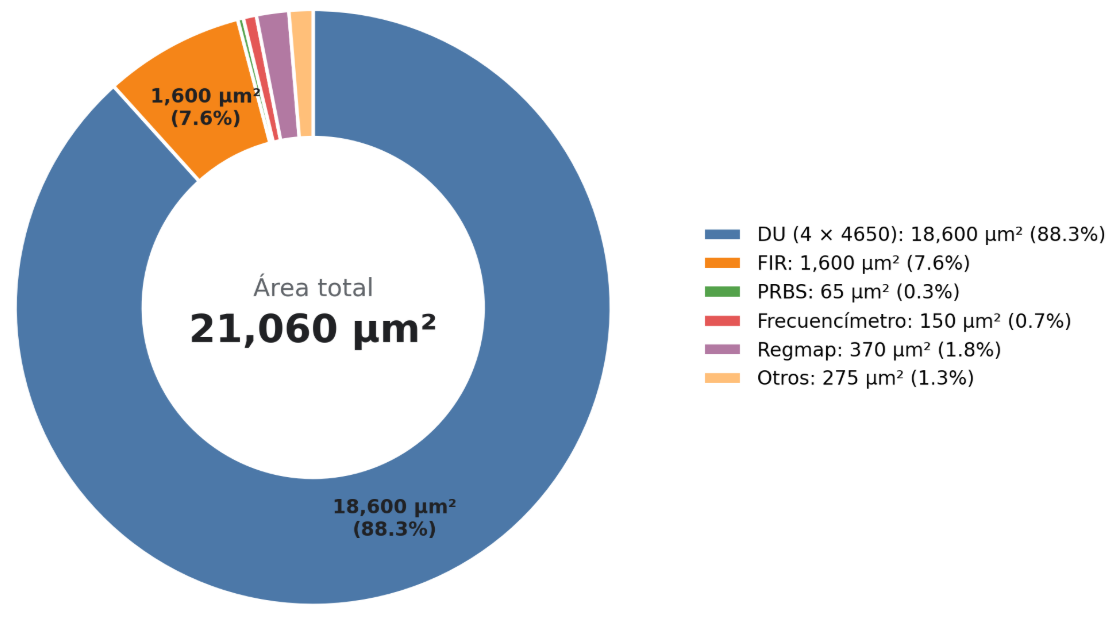
\includegraphics[width=0.92\linewidth]{area.png}
    \caption{Distribución del área sintetizada entre los bloques del sistema.}
    \label{fig:top-area}
\end{figure}

\subsubsection*{Potencia}

La Tabla~\ref{tab:top-power} resume el reporte de potencia total, entre los principales
bloques.

\begin{table}[H]
    \centering
    \caption{Potencia estimada para el sistema integrado.}
    \label{tab:top-power}
    \begin{tabular}{@{}lrr@{}}
        \toprule
        \textbf{Bloque} & \textbf{Potencia} & \textbf{Proporción} \\
        \midrule
        DU     & 1.2mW & 68.5\%\\
        Others & 0.55mW & 31.5\% \\
        \midrule
        Total        & 1.75mW & 100\%\\
        \bottomrule
    \end{tabular}
\end{table}

\subsubsection*{Distribución de celdas por tensión de umbral}

La proporción de celdas según su tensión de umbral permite analizar el compromiso
realizado por la herramienta entre velocidad y potencia. Las celdas de menor tensión 
de umbral ofrecen mayor velocidad a costa de un mayor leakage, mientras que las de 
mayor tensión de umbral reducen el leakage pero son más lentas.

\begin{table}[H]
    \centering
    \caption{Distribución de celdas según su tensión de umbral.}
    \label{tab:top-vt}
    \begin{tabular}{@{}lrr@{}}
        \toprule
        \textbf{Tipo de celda} & \textbf{Cantidad} & \textbf{Proporción} \\
        \midrule
        HVT  & 26009 & 98.7\% \\
        RVT  & 15    & 0.06\% \\
        LVT  & 304   & 1.15\% \\
        SLVT & 21    & 0.08\% \\
        \midrule
        Total & 26349 & 100\% \\
        \bottomrule
    \end{tabular}
\end{table}

% ---------------------------------------------------------------------------
\section{Conclusiones}
\label{sec:conclusiones}
% ---------------------------------------------------------------------------

En este trabajo se diseñaron y verificaron los distintos bloques que componen el
sistema, para luego integrarlos en un único módulo \texttt{top}. La arquitectura
obtenida permite generar una secuencia PRBS paralela, convertirla a PAM-2,
procesarla mediante un filtro FIR y capturar sus cuatro salidas utilizando las
DUs. A su vez, el mapa de registros permite configurar y controlar el sistema
desde el dominio CPU, mientras que el frecuencímetro permite comprobar la
frecuencia del clock DSP.

Los resultados obtenidos fueron satisfactorios. Las simulaciones presentaron un
comportamiento acorde con el funcionamiento diseñado y esperado, tanto para cada
bloque como para el sistema completo. Los resultados de síntesis también fueron 
satisfactorios: el diseño cumple las restricciones de timing para los clocks de 
1~GHz y 200~MHz, con valores de área y potencia razonables para los distintos 
bloques del sistema. El área se encuentra dominada por las cuatro DUs debido a 
sus memorias, mientras que la potencia total estimada es de 1,75~mW. Por otro 
lado, resulta llamativa la elevada proporción de celdas HVT. Esto podría indicar 
que existe margen para cerrar timing a frecuencias mayores, aunque evaluar ese 
límite no forma parte del objetivo de este trabajo.

La principal dificultad encontrada consistió en dejar de considerar cada bloque
como una caja negra y comenzar a pensarlo como parte de un sistema completo. Esto
requirió tener en cuenta en qué momento y de qué manera se configura cada módulo,
además de la relación entre sus señales de control y de datos. La existencia de
dominios de clock diferentes para la configuración y el datapath agregó
complejidad a estas transacciones.

Como posible mejora, sería interesante evaluar una tecnología que permita inferir
memorias en lugar de implementar el almacenamiento mediante grandes bancos de
registros. Esto permitiría comprobar si es posible reducir el área y la potencia
de las DUs, que constituyen el bloque dominante en ambas métricas.

El balance final del trabajo es muy positivo, ya que permitió comprender mejor el
funcionamiento de un ASIC desde una perspectiva global y tomar decisiones de
diseño desde las primeras etapas, considerando su impacto sobre el
funcionamiento del sistema como un todo.

\end{document}
